\documentclass{article}
\usepackage{algorithm}
\usepackage{algpseudocode}
\usepackage{amsmath,amssymb,amsthm}
\usepackage{graphicx}
\usepackage[margin=1in]{geometry}
\usepackage{fancyhdr}
\usepackage{float}
\usepackage{longtable}
\setlength{\parindent}{0pt}
\setlength{\parskip}{5pt plus 1pt}
\setlength{\headheight}{13.6pt}
\newcommand\question[2]{\vspace{.25in}\hrule\textbf{#1: #2}\hrule\vspace{.10in}}
\renewcommand\part[1]{\vspace{.10in}\textbf{(#1)}}
\newcommand\algo{\vspace{.10in}\textbf{Algorithm: }}
\newcommand\correctness{\vspace{.10in}\textbf{Correctness: }}
\newcommand\runtime{\vspace{.10in}\textbf{Running time: }}
\newcommand\pseudoCode{\vspace{.10in}\textbf{PseudoCode: }}
\newcommand*{\perm}[2]{{}^{#1}\!P_{#2}}
\newcommand*{\comb}[2]{{}^{#1}\!C_{#2}}
%\pagestyle{fancyplain}
%\lhead{\textbf{\NAME\ (\UID)}}
%\chead{\textbf{Hw\HWNUM}}
%\rhead{CS 6350, \today}
\title{CS6350 - Homework/Assignment-5}
\author{Arnab Das(u1014840)}
\usepackage[utf8]{inputenc}
\begin{document}
  \pagenumbering{gobble}
  \maketitle
  \newpage
  \pagenumbering{arabic}
  \newcommand\NAME{ARNAB DAS}
  \newcommand\UID{uxxxxxxx}
  \newcommand\HWNUM{4}

  \question{1}{Margins}
  \part{1} For a xor function in two dimension of $x_{1},x_{2}$ and label $y$, the examples sets in the form of tuple $(x_1, x_2, y)$ are $(-1,-1,-1)$, $(-1,1,1)$, $(1,-1,1)$ and $(1,1,-1)$, where variables are boolean and takes $\{-1,1\}$. It is not linearly separable in the euclidean space. However, the transformation, $\phi$, of mapping $[x_1, x_2]$ to $[x_1, x_1x_2]$ makes it linearly separable in which the datapoints now $(x_1, x_1x_2, y)$ becomes $(-1,1,-1)$, $(-1,-1,1)$, $(1,-1,1)$ and $(1,1,-1)$. The line $x_1x_2=0$ is a separating classifier. SInce $x_1x_2=0$ is equaidistant from all the 4 points in the transformed space, it gives the maximum margin, which is the distance of any of the points(since equidistant) from this line. and equal to \textbf {1 unit}.  The linear classifier in the transformed space when mapped back to the original euclidean space , will be combination of the lines $x_1=0$ and $x_2=0$, as shown in Figure-1(c). This is because in the transformed space, since $x_1x_2=0$ means that line satisfies all points which has $x_1=0$ or/and $x_2=0$, hence in the euclidean space it is a combination of both. \newline

  \begin{figure}[H]
   \centering
  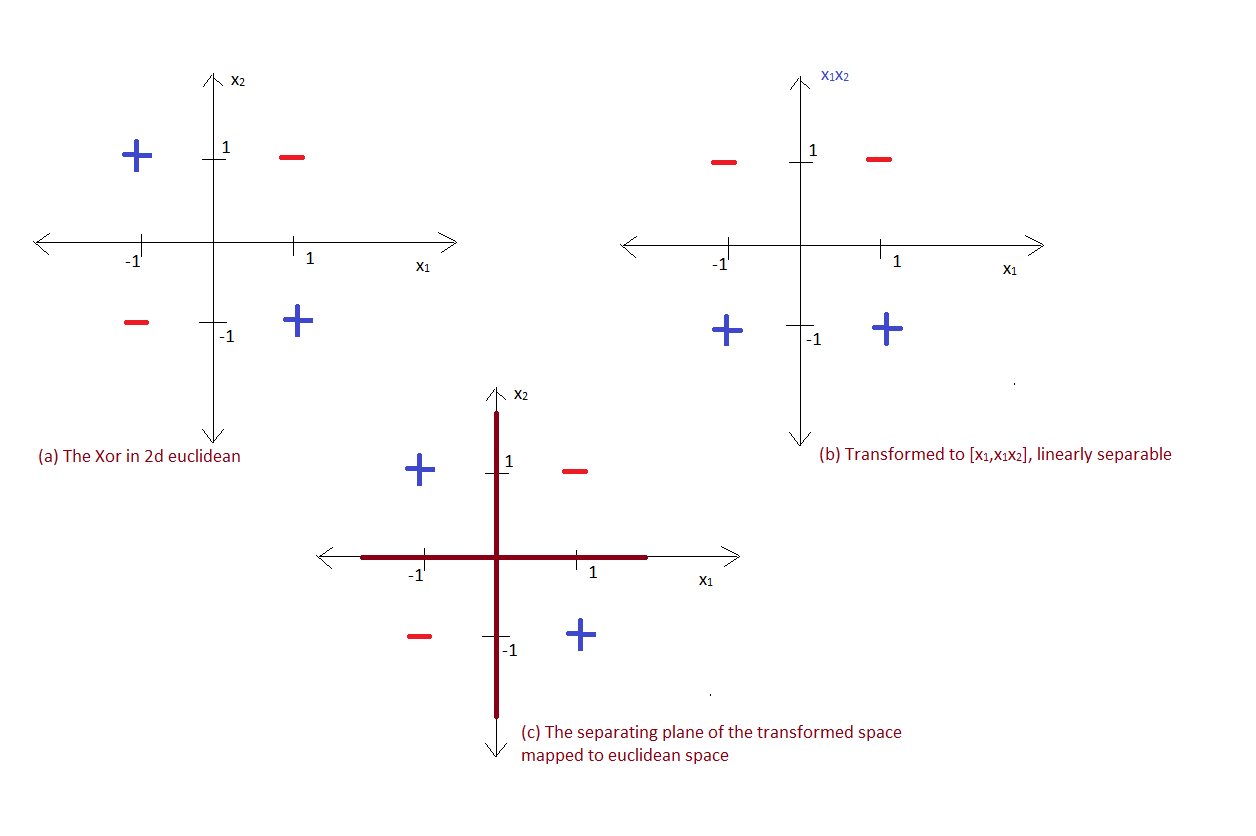
\includegraphics[width=12cm, height=12cm]{Prob1a}
  \caption{Space transformation for Xor to make linearly separable}
  \end{figure}

  \part{2a} For $D_1 = \{x_1, x_2, x_3, x_5, x_7\}$, the linear classifier with the maximum margin will be parallel to the line joining $x_1$ and $x_3$, and the distance of this classifer will be equal from $x_1 and x_3$ on one side and $x_5$ on the other side.  Hence, the maximum possible margin for $D_1$ will be half the distance of $x_5$ from the line joining $x_1$ and $x_3$. The line joining $x_1,x_3$ is $x_1 - x_2 = 0$. Then, margin for $D_1$ will be: \newline
  \[D_{1_{marginMax}} = \dfrac{1}{2 \times \sqrt[2]{2}}\]
 
    For $D_2 = \{ x_1, x_5, x_6, x_8\}$, the linear classifier with the maximum margin will be parallel to the line joining $x_5, x_6$, and the distance of this classifier will be equal from $x_5$ and $x_6$ on one side and $x_1$ on the other side. Hence, the maximum possible margin for $D_2$ will be half of the distance of $x_1$ from the line joining $x_5$ and $x_6$. The line joining $x_5, x_6$ is $\sqrt[2]{3}x_1 + x_2 - \sqrt[2]{3} = 0$. Then the margin for $D_2$ will be: \newline
    \[D_{2_{marginMax}} = \dfrac{\sqrt[2]{3}}{4} \]

    For $D_3 = \{ x_3, x_4, x_5, x_7 \}$, the linear classifier with the maximum margin will be parallel to the line joining $x_4$ and $x_3$, and the distance of this classifier will be equal from $x_4$ and $x_3$ from one side and from $x_5$ on the other side. Hence, the maximum possible margin for $D_3$ will be half of the distance of $x_5$ from the line joining $x_3$ and $x_4$. The line joining $x_3$ and $x_4$ is $2x_1 - x_2 - 1 = 0$. Then the margin for $D_3$ will be: \newline
    \[ D_{3_{marginMax}} = \dfrac{1}{2\times \sqrt[2]{5}}\]

    \part{2b}
    For finding the perceptron mistake bound, the mistake bound is given as $\leq \bigg ( \dfrac{R}{\gamma} \bigg )^2$, where is the farthest point from the origin. \newline
    For $D_1$, farthest point is $x_7$, so $R=\dfrac{3}{2}$ and $\gamma = \dfrac{1}{2 \times \sqrt[2]{2}}$, perceptron mistake bound for $D_1$ = 18. \newline
    For $D_2$, farthest point is $x_8$, so $R=\dfrac{\sqrt[2]{5}}{2}$ and $\gamma=\dfrac{\sqrt[2]{3}}{4}$, perceptron mistake bound for $D_2$ = 6 $\leq \dfrac{20}{3}$. \newline
    For $D_3$, farthest point is $x_7$, so $R=\dfrac{3}{2}$ and $\gamma = \dfrac{1}{2\times \sqrt[2]{5}}$, perceptron mistake bound for $D_3$ = 45. \newline
    $D_3$ has the greatest mistake bound. \newline

    \part{2c} A higher mistake bound indicates how well the classifier can fit the training data by making only this bounded number of mistakes. Hence, a low mistake bound will means the classifier fits the training data quickly. However, that provides no guarantees on the test data. Since the perceptron learns by making mistakes, hence a lower number of mistakes indicate that the learning performed by the perceptron has been less, and hence its predictive power intuitively reduces on the test data. To put it simply, a classifier learns less if it makes less number of mistakes because that is its only entry point towards learning and updates. Hence, the classifier with a higher mistakes bound is easier to learn and the one with a small mistake bound is difficult to learn. Thus the ranking in order of ease of ranking will be $D_3$, $D_1$, $D_2$ . \newline

    \question{2}{Kernels}
    \part{1a} Given valid kernels , $K_1(x,z)$ and $K_2(x,z)$, we need to show the product of these two kernels is also a kernel. For the defined space $x_1, x_2, \dots, x_n \in S$, we define the respective Gram matrices as: \newline
    \[ C = \{c_{ij}\} = K_1(x_i, x_j) \]
    \[ D = \{d_{ij}\} = K_2(x_i, x_j) \]
    We define the newKernel $K=K_1 \times K_2$ as the product of these kernels , such that its Gram matrix looks like: \newline
    \[ E = \{e_{ij}\} = \{c_{ij}\}\{d_{ij}\} = K(x_i, x_j) \]

    Now, since the kernels $K_1$ and $K_2$ are spd, hence the elements are symmetric. So , we can write : \newline
    \[ C = \{c_{ij}\} = K_1(x_i, x_j) = \{c_{ji}\} = K_1(x_j, x_i) \]
    \[ D = \{d_{ij}\} = K_2(x_i, x_j) = \{d_{ji}\} = K_2(x_j, x_i) \]
    Then , the corresponding elements in the matric for the new kernel, will be:
    \[ \{e_{ji}\} = \{c_{ji}\}\{d_{ji}\} = \{c_{ij}\}\{d_{ij}\} = \{e_{ij}\}  \]
    \textbf {Hence, the new kernel is also symmetric. }
    Now, we need to prove it is symmetric positive definite. Let $u \in R^n$, we need to show $u^TEu \geq 0$. We can write:\newline
    \begin{equation}
    u^TEu = \sum_{ij} u_i u_j e_{ij} = \sum_{ij} u_i u_j c_{ij} d_{ij}
    \end{equation}

    Now, any matrix A that is non-singular, can be turned into a symmetric positive definite matrix by multiplication with its transpose, that is $A^TA$ is always symmetric positive definite. Since, the matrix A can be any matrix without any restriction other than being non-singular, this means that a given symmetric positive definite matrix can be considered to be formed as a product of  matrix and its transpose. So, we break down C as a product of a general non-singular matrix A and its transpose, and D as the product of a general non-singullar matrix B and its transpose. 
    \[C = A^TA = \{c_{ij}\} = a_{i}^Ta_j = \sum_{k} a_{ik}a_{jk} \]
    \[D = B^TB = \{d_{ij}\} = b_{i}^Tb_j = \sum_{l} b_{il}b_{jl} \]
   Plugging these back to equation(1), we get: 
    \[u^TEu = \sum_{ij} u_i u_j e_{ij} = \sum_{ij} u_i u_j \sum_{k} a_{ik}a_{jk} \sum_{l} b_{il}b_{jl} =\sum_{kl} \sum_{ij} u_i u_j a_{ik}a_{jk} b_{il}b_{jl}\] 
    \[u^TEu = \sum_{kl} \sum_{ij} u_i u_j a_{ik} a_{jk} b_{il} b_{jl}\]
    Since the i,j do not depend on each other, we can separate these as below
    \[u^TEu = \sum_{kl} ( \sum_{i} u_i a_{ik} b_{il}) (\sum_{j} u_j a_{jk} b_{jl})\]
    The terms for j are completely independent of i, and exactly identical to i, so we can remove the j terms and place the i terms as square which is greater than equal to 0
    \[u^TEu = \sum_{kl} ( \sum_{i} u_i a_{ik} b_{il})^2 \geq 0\]
    Hence, the gram matrix E is symmetric positive definite, which means K is also a kernel.(Proved). \newline

    \part{2a} To Prove: Polynomial over a kernel constructed using positive coefficients is also a kernel.\newline
    If we can show that the sum of kernels with positive coefficients is a kernel, then using this result and the result of previous question(2.1.a), we can conclude that Polynomial over a kernel is also a kernel. \newline
    Given $K_1(x,z)$ and $K_2(x,z)$ are kernels, we define $K(x,z) = \alpha K_1(x,z) + \beta K_2(x,z)$ and show that K is a kernel. \newline
    Suppose $K_1$ has its feature map, $\phi_1$, such that it is defined as $K_1(x,z) = \phi_1^T(x)\phi_1(z)$.
    Suppose $K_2$ has its feature map, $\phi_2$, such that it is defined as $K_1(x,z) = \phi_2^T(x)\phi_2(z)$. Then we have , \newline
    \[K(x,z) = \alpha K_1(x,z) + \beta K_2(x,z) = <\sqrt[2]{\alpha}\phi_1(x), \sqrt[2]{\alpha}\phi_1(z)> + <\sqrt[2]{\beta}\phi_1(x), \sqrt[2]{\beta}\phi_1(z)>\]
    \[K(x,z) = <[\sqrt[2]{\alpha}\phi_1(x), \sqrt[2]{\beta}\phi_2(x)], [\sqrt[2]{\alpha}\phi_1(z), \sqrt[2]{\beta}\phi_2(z)]>\]

    Which means $K(x,z)$ can be expresses as an inner product . Hence, K is an kernel.
    Next, when we have a polynomial over a kernel constrcuted using positive coefficients, then the terms of the polynomial are product of kernels and these products are summed up to produce the final polynomial. Since, we have already proved that the product of kernels is a kernel, and sum of kernels with positive(else $\sqrt[2]{\alpha}$ will be imaginary) coefficients are kernels, hence overall it is a kernel. (Proved). \newline

    \part{2} Given two examples $x \in R^2$ and $z \in R^2$, \textbf {Prove} the following is a kernel.
    \[K(x,z) = 15(x^Tz)^2 \exp(-||x-z||^2)\]
    Let $K_1(x,z) = 15(x^Tz)^2$ and $K_2 = \exp(-||x-z||^2)$. We already know from the previous results that the product of two kernels is a kernel. Hence, if we can separately prove that $K_1$ and $K_2$ are kernels, then that implies K is a kernel as well. \newline
    \textbf {Proof: $K_1$ is a kernel: } Mercer's condition says, K is a valid if for every finite set ${x_1, x_2, \dots, x_n}$, for any choice of real valued $c_1, c_2, \dots$, if $\sum_i \sum_j K(x_i,x_j) \geq 0$. Choosing $c_i,c_j$ to be positive real values, then for any pair of examples $x_i.x_j$, for $K_1$, we can write: $\sum_i \sum_j c_i c_j 15(x^Tz)^2$, and since their is a square term involved with positive coefficients, hence its value is greater than equal to 0. Thus , $K_1$ is a valid kernel. \newline
    \textbf {Proof: $K_2$ is a kernel: }. We can break down $K_2$ as follows:
    \[K_2(x,z) = \exp(-||x-z||^2) = \exp(-(x-z)^T(x-z)) = \exp(-<x-z, x-z>) = \exp(-(<x,x-z> - <z,x-z>)) \]
    \[K_2(x,z) = \exp(-(<x,x> - <x,z> - <z,x> + <z,z>)) = \exp(-(||x||^2 + ||z||^2 - 2<x,z>))\]
    \[K_2(x,z) = \exp(-(||x||^2 + ||z||^2)) \exp(2<x,z>) = C\exp(2<x,z>)\]
    where C = $\exp(||x||^2 + ||z||^2)$ is a constant. Then expanding the exponential we get:
    \begin{equation}
    K_2(x,z) = C \sum_{n=0}^\infty \dfrac{<x,z>^n}{n!}
    \end{equation}

    Thus, we see that $K_2$ is formed by an infinite sum over polynomial kernels, which are further derived from the product of linear kernels$x^Tz$. Since sum and product of kernels results in a kernel as proved earlier, hence $K_2$ is a kernel. \newline
    Since, $K$ is formed as the product of $K_1$ and $K_2$, hence $K_1$ is a valid kernel.(Proved). \newline

    \part{3} Prove that the Gaussian kernel can be written down as the inner product of an feature space with infinite dimension. 
    \[K(x,z) = \exp(\dfrac{-||x-z||^2}{2{\sigma}^2})\]

    Continuing from Equation(2) of the above proof and using the earlier proofs as well: \newline
    Since, we can write the sum of two kernels as a new kernel, such that
    \[K(x,z) = K_1(x,z) + K_2(x,z)\]
    and their corresponding transformations be $\phi$ , $\phi_1$ and $\phi_2$ respectively. This implies that $\phi$ is defined such that it forms vectors of the form:
    \[ \phi(x) = (\phi_1(x), \phi_2(x))\]
    such that(similar to the proof for sum over kernels)
   \[ <\phi(x),\phi(z)> = <\phi_1(x), \phi_1(z)> + <\phi_2(x), \phi_2(z)>\]
   In the euclidean space, thus $\phi(x)$ is the vector formed by appending the components of $\phi_2(x)$ to $\phi_1(x)$, and then:
   \[<\phi(x), \phi(z)> = \sum_{i=1}^{dim(K_1)} \phi_{1,i}(x)\phi_{1,i}(z) + \sum_{j=1}^{dim(K_2)} \phi_{1,j}(x)\phi_{1,j}(z)\]
   \[ = \sum_{i=1}^{dim(K_1)+dim(K_2)} \phi_{i}(x)\phi_{j}(z)\]

   Since $K_1$ and $K_2$ are infinite sum over kernel polynomials from equation(2), hence $K$ can be written down as the inner product of a feature space with infinite dimension as shown above. Here, $K$ represents the RBF, while $K_1$ and $K_2$ represents the infinite sums RBF is composed off as in equation(2). \newline

   \question{3.1}{Support Vector Machines}
   \part{1} Implementation of SVM with $C=1$ and $\gamma_0 = 0.01$. \newline
   DataSet = Handwriting \newline
   Training Accuracy = 94.1\% \newline
   Test Accuracy = 91.9\% \newline

   \part{2} Below table reports the results of the 5-fold experiments on the madelon dataset across varying values for $C$ and $\gamma_0$
  
 \begin{longtable}{c|c|c|c}
  \caption{5-fold experiment on Madelon data set} \\
  %\centering
  %\begin{tabular}{c c  c c }
  \hline\hline
	  C & $\gamma_0$ & Avg.Training Accuracy($\%$) & Avg.Test Accuracy($\%$) \\[1ex]
  \hline
	  1 & 1 & 53.95 & 50.0 \\
	  1 & 0.1 & 54.95 & 51.1 \\
	  1 & 0.01 & 52.91 & 49.2 \\
	  1 & 0.001 & 54.88 & 52.45 \\
	  1 & 0.0001 & 59.18 & 53.95 \\
	  1 & 10 & 55.93 & 51.8 \\
	  1 & 100 & 57.48 & 55.15 \\
	  2 & 1 & 55.16 & 52.3 \\
	  2 & 0.1 & 53.76 & 52.95 \\
	  2 & 0.01 & 56.9 & 52.75 \\
	  2 & 0.001 & 53.575 & 51.15 \\
	  2 & 0.0001 & 52.775 & 52.7 \\
	  2 & 10 & 53.975 & 50.75 \\
	  2 & 100 & 54.01 & 51.3 \\
	  0.5 & 1 & 59.73 & 52.95 \\
	  0.5 & 0.1 & 52.47 & 49.9 \\
	  0.5 & 0.01 & 64.01 & 55.95 \\
	  0.5 & 0.001 & 57.83 & 52.7 \\
	  0.5 & 0.0001 & 54.71 & 51.45 \\
	  0.5 & 10 & 57.75 & 53.0 \\
	  0.5 & 100 & 58.61 & 51.7 \\
	  0.25 & 1 & 60.57 & 54.55 \\
	  0.25 & 0.1 & 59.85 & 54.4 \\
	  0.25 & 0.01 & 54.08 & 50.35 \\
	  0.25 & 0.001 & 56.63 & 53.45 \\
	  0.25 & 0.0001 & 65.65 & 56.85 \\
	  0.25 & 10 & 58.6625 & 52.55 \\
	  0.25 & 100 & 61.52 & 52.0 \\
	  0.0625 & 1 & 55.23 & 55.1 \\
	  0.0625 & 0.1 & 57.38 & 53.8 \\
	  0.0625 & 0.01 & 59.71 & 54.0 \\
	  0.0625 & 0.001 & 62.31 & 56.35 \\
	  0.0625 & 0.0001 & 61.78 & 53.25 \\
	  0.0625 & 10 & 56.85 & 55.0 \\
	  0.0625 & 100 & 55.63 & 51.6 \\
	  4 & 1 & 51.5 & 50.15 \\
	  4 & 0.1 & 54.21 & 50.1 \\
	  4 & 0.01 & 50.81 & 49.05 \\
	  4 & 0.001 & 55.32 & 54.7 \\
	  4 & 0.0001 & 54.96 & 52.8 \\
	  4 & 10 & 55.32 & 52.2 \\
	  4 & 100 & 54.16 & 53.65 \\
	  0.01 & 1 & 57.52 & 53.95 \\
	  0.01 & 0.1 & 57.63 & 55.75 \\
	  0.01 & 0.01 & 58.87 & 56.8 \\
	  0.01 & 0.001 & 62.1 & 57.6 \\
	  0.01 & 0.0001 & 61.85 & 56.55 \\
	  0.01 & 10 & 57.7 & 56.05 \\
	  0.01 & 100 & 56.87 & 54.9 \\
	  0.1 & 1 & 56.87 & 53.3 \\
	  0.1 & 0.1 & 57.43 & 53.15 \\
	  0.1 & 0.01 & 58.97 & 52.0 \\
	  0.1 & 0.001 & 59.4 & 53.35 \\
	  0.1 & 0.0001 & 62.71 & 53.2 \\
	  0.1 & 10 & 57.82 & 56.2 \\
	  0.1 & 100 & 56.2 & 51.7 \\ [1ex]
  %\end{tabular}
  %\label{table:nonlin}
  \end{longtable}

  The C list on trial = $[1, 2, 0.5, 0.25, 0.0625, 4, 0.01, 0.1]$ \newline
  The $\gamma_0$ list on trial = $[1, 0.1, 0.01, 0.001, 0.0001, 10, 100]$ \newline
  From the experiment , the final extracted best combinations of hyperparameyters and corresponding accuracy are listed below: \newline
  Best C = 0.01 \newline
  Best $\gamma_0$ = 0.001 \newline
  \textbf {Training:} Accuracy = 61.1\% \newline
  \textbf {Test:} Accuracy = 58.66\% \newline

  \part{3} Precision, Recall and F1 scores.\newline
  \textbf {Handwriting Data Set}: \newline
  \textbf {Training:} Precision Score = 0.925 \newline
  \textbf {Training:} Recall Score = 0.970 \newline
  \textbf {Training:} F1-Score = 0.947 \newline
  \textbf {Test:} Precision Score = 0.90 \newline
  \textbf {Test:} Recall Score = 0.947 \newline
  \textbf {Test:} F1-Score = 0.923 \newline

  \textbf {Madelon Data Set}: \newline
  \textbf {Training:} Precision Score = 0.73 \newline
  \textbf {Training:} Recall Score = 0.352 \newline
  \textbf {Training:} F1-Score = 0.475 \newline
  \textbf {Test:} Precision Score = 0.69 \newline
  \textbf {Test:} Recall Score = 0.313 \newline
  \textbf {Test:} F1-Score = 0.43 \newline

  \question{3.2}{Ensemble of Decision Trees}
  \part{1} Creating an N ensemble decision tree whose output forms an N dimensional input vector to a SVM classifier. Here we test on N=(5,10,100), and $C = 0.1$, $\gamma_0 = 0.01$ and epochs = 60. The value of k, the randomly selected features at every split = $\log_2d = \log_2256 = 8$. The results are reported below in Table-2: \newline

 \begin{longtable}{c|c|c|c|c|c|c|c|c}
  \caption{5-fold experiment on Madelon data set} \\
  %\centering
  \hline\hline
	  N & Train-Acc$\%$ & Train-Prec & Train-Recall & Train-F1 & Test-Acc$\%$ & Test-Prec & Test-Recall & Test-F1 \\[0.5ex]

  \hline
	 5 & 99.4 & 0.99 & 0.99 & 0.99 & 86 & 0.91 & 0.80 & 0.85 \\
	 10 & 100 & 1 & 1 & 1 & 88.87 & 0.95 & 0.82 & 0.88 \\
	 100 & 100 & 1 & 1 & 1 & 90.21 & 0.95 & 0.84 & 0.89 \\ [0.5ex]
  %\end{tabular}
  %\label{table:nonlin}
  \end{longtable}

  \part{2} For implementing the ensemble method on the madelon dataset, we need to discretize the data from the continuous domain. For this we choose the following split method. At every node, we select k random features. For each feature f, we collect its values across the examples and its labels. Then this map list is sorted, and split points are identified wherever the label changes sign. These split points are identified as a threshold value. Based on this identified split points, we calculate the information gain(based on entrophy) and choose the split for that feature that provided the best information gain, and that infromation gain is the representative of that feature in the decision function that needs to make a decision across the randomly selected k features.  So, once the split splot for each feature has been identified, the feature with the best split/cut (highest information gain), is chosen as the feature to split upon. Once, this decision  has been made,the branching from that node has two branches, one for samples with the corresponding value greater than or equal to threshold and the other for less than threshold. Then at the node in the next level, we have atleast one less feature to split from. We again select random k features, for the duration the available features to split on is greater than or equal to k. Once the available features to split on becomes equal to k, we random selection goes off and we select all the features. \newline
  The choice of the number of examples(m) we take to train each decision tree plays a crucial role here. Our experiments show that with higher values of m, the trees overfit the data and training accuracy shoots up, while the test accuracy goes down. This is precisely because we developed \textbf {unpruned} trees, which will fit the entire training set. To reduce overfitting, we decided to limit the value of 'm' samples that goes to each decision tree. For $n$ being the number of decision trees, and $D$ being the length of the input data set, we chose $m = \dfrac{D}{p*n}$. The m samples are chosen randomly for each decision tree and with replacement. Our trials with $p=1,2,5$, shows that around $p=1,2$ results are fairly optimal. With $p=5$, the results starts to drift away indicating underfitting since we are not supplying enough examples to train upon. Besides, we have tried with setting $m={25\%, 50\%, 70\%}$ of the data set. While $25\%$ gave a similar accuracy as $p=1$ for n=5, that is expected since they both points towards similar sample size. Increasing the percentage of the data-set in the sample improved training-accuracy to around $80\%$ while test-accuracy drops off to lower 40's, indicating too much overfitting. \newline

  Values used for $(C,\gamma_0) = (1,0.01)$. This is the best we got after many trial runs for accuracy. \newline
 \begin{longtable}{c|c|c|c|c|c|c|c|c|c}
  \caption{Ensemble experiment on handwriting data set} \\
  %\centering
  \hline\hline
	  N & p & Train-Acc$\%$ & Train-Prec & Train-Recall & Train-F1 & Test-Acc$\%$ & Test-Prec & Test-Recall & Test-F1 \\[0.5ex]

  \hline
	 5 & 1 & 68.85 & 0.68 & 0.68 & 0.68 & 52 & 0.60 & 0.112 & 0.19 \\
	 10 & 1 & 70.8 & 0.70 & 0.71 & 0.70 & 52.66 & 0.58 & 0.18 & 0.27 \\
	 30 & 1 & 72.85 & 0.72 & 0.73 & 0.73 & 52.33 & 0.55 & 0.22 & 0.31 \\
	 100 & 1 & 73.25 & 0.74 & 0.71 & 0.72 & 49.83 & 0.49 & 0.19 & 0.27 \\
	 5 & 2 & 60.65 & 0.60 & 0.63 & 0.61 & 52 & 0.51 & 0.76 & 0.61 \\
	 10 & 2 & 61.35 & 0.60 & 0.66 & 0.63 & 51.5 & 0.51 & 0.76 & 0.61 \\
	 30 & 2 & 62.6 & 0.61 & 0.65 & 0.63 & 50 & 0.5 & 0.67 & 0.57 \\
	 100 & 5 & 65.8 & 0.66 & 0.63 & 0.64 & 49.33 & 0.49 & 0.66 & 0.56 \\
	 5 & 5 & 54.4 & 0.54 & 0.58 & 0.56 & 46.33 & 0.456 & 0.386 & 0.418 \\
	 10 & 5 & 56 & 0.55 & 0.65 & 0.59 & 46.33 & 0.421 & 0.196 & 0.268 \\
	 30 & 5 & 59.5 & 0.57 & 0.69 & 0.63 & 47 & 0.47 & 0.48 & 0.47 \\
	 100 & 5 & 62.8 & 0.61 & 0.70 & 0.65 & 46 & 0.45 & 0.39 & 0.419 \\ [0.5ex]
  %\end{tabular}
  %\label{table:nonlin}
  \end{longtable}
  
   
   The best choice of N(number of decision trees) comes to be 10 with p=1. Below is the reported accyracy and precision,recall scores. \newline
     \textbf {N=10, p=1, C=1, $\gamma_0$=0.01} \newline
     \textbf {Training: } Accuracy = 70.8\% \newline
     \textbf {Training: } Precision = 0.70 \newline
     \textbf {Training: } Recall = 0.71 \newline
     \textbf {Training: } F1-Score = 0.70 \newline

     \textbf {Test: } Accuracy = 52.66\% \newline
     \textbf {Test: } Precision = 0.58 \newline
     \textbf {Test: } Recall = 0.18 \newline
     \textbf {Test: } F1-Score = 0.27 \newline

\end{document}
